% !TEX program = xelatex
% 會議論文草稿（中文版）-- Gary Wang
% 目標期刊：EMBC 2026 / AMIA 2026 / EMNLP 2026 Clinical NLP

\documentclass[12pt, a4paper]{article}
\usepackage[fontset=none]{ctex}
\setCJKmainfont{Microsoft JhengHei}
\setCJKsansfont{Microsoft JhengHei}
\setCJKmonofont{Microsoft JhengHei}

\usepackage{amsmath}
\usepackage{amssymb}
\usepackage{graphicx}
\usepackage{booktabs}
\usepackage[table]{xcolor}
\usepackage{hyperref}
\usepackage{array}
\usepackage{microtype}
\usepackage{geometry}
\usepackage{authblk}
\usepackage{caption}
\usepackage{enumitem}

\geometry{top=2.5cm, bottom=2.5cm, left=3cm, right=3cm}

\hypersetup{
    colorlinks=true,
    linkcolor=blue,
    citecolor=blue,
    urlcolor=blue
}

\graphicspath{{../../result/multi_model_results/pdf/}{../../feature_selection/wrapper_vs_mlp_results/}{../../feature_selection/fs_results_v2/pdf/}{../../result/fs_results/pdf/}}

% -------------------------------------------------------
\title{\textbf{基於大型語言模型的 MDS-UPDRS 手指敲擊嚴重度評分：\\以節省 Token 的特徵選取為基礎}}

\author[1]{Gary Wang}
\affil[1]{Nordling Lab，國立成功大學機械工程學系，台南 70101，台灣\\
\texttt{gary.wang@nordlinglab.org}}

\date{}

% -------------------------------------------------------
\begin{document}

\maketitle

% -------------------------------------------------------
\begin{abstract}
先前基於大型語言模型（LLM）的臨床動作評估方法，將原始運動學軌跡 CSV 資料（每 session 約 2\,400 列）直接塞入提示詞，每次查詢的 session 資料消耗約 15\,000 個 token，且須仰賴大型專有模型。本文提出一種節省 token 的替代方案，結合多方法共識特徵選取與少樣本提示：利用 CoTracker 軌跡追蹤萃取 149 個運動學特徵後，透過 28 種特徵選取方法的交叉選頻共識濃縮至 7 個特徵子集，將總提示詞從 $\sim$15\,000 個 token 壓縮至約 400 個 token（零樣本）——\textbf{減少 97\%}。應用於 MDS-UPDRS 手指敲擊嚴重度自動評分（$n$\,=\,53 個 session，來自 16 位帕金森氏症患者），此精簡輸入使僅有 32B 參數的開源模型能夠超越同一資料集上 GPT-4 的最佳結果。最佳配置（Deepseek-R1-32B，少樣本）達到 MAE\,=\,0.36、加權 $\kappa$\,=\,0.68、相鄰準確率\,=\,98\%——與人類專家 MAE 相當，並接近評分者間 $\kappa$（0.69--0.83）。在二元篩選任務（正常 vs.\ 異常敲擊），DS-R1-32B 少樣本達到 100\% 召回率，零漏判。本研究顯示，預先萃取特徵可同時取代原始軌跡輸入與大型專有模型，實現具成本效益且保護隱私的臨床評估。

\noindent\textbf{關鍵詞：}特徵選取共識、帕金森氏症、MDS-UPDRS、token 效率、臨床自然語言處理
\end{abstract}

% -------------------------------------------------------
\section{簡介}

帕金森氏症（PD）是一種進行性神經退化疾病，2021 年全球約有 1\,180 萬名患者——相較 1990 年增加了 274\%~\cite{steinmetz2024global}。遲緩動作（bradykinesia）是其核心運動症狀，臨床上以 MDS-UPDRS 第三部分手指敲擊子測驗（項目 3.4）進行量化，依速度、幅度、節律與停頓評分為 0 至 4 分~\cite{cite_updrs}。由於此評估需要受過訓練的動作障礙專科醫師，在資源受限的場域中可及性有限，催生了自動化評分工具的需求。

先前的機器學習方法萃取工程化運動學特徵（頻率、幅度、週期變異），並輸入 SVM、隨機森林或 LightGBM 等分類器~\cite{cite_ml_motor,cite_ml_motor2,yang2024deep}。雖然能捕捉統計模式，這些模型需要數百筆標注樣本才能可靠訓練，且缺乏整合特定領域臨床推理的能力~\cite{sarker2022ai}。LLM 則在大量醫學文獻上訓練，能透過臨床指引的視角解讀結構化特徵資料，並在預測旁附上逐步推理過程~\cite{minaee2024large}——此優勢在臨床手指敲擊研究常見的小樣本資料集中尤為突出。

最直接的 LLM 前驅研究為 Chen~\cite{chen2024chatgpt}，其將\emph{原始 2\,400 列 CSV 軌跡資料與 Python 特徵萃取腳本}直接寫入 ChatGPT-4 提示詞。此方法每次推論需消耗約 15\,000 個 session token，四樣本少樣本變體（Experiment~D）更高達約 75\,800 個 token，達到 ICC(2,1)\,=\,0.45——該資料集上迄今最佳的 LLM 結果。然而對前沿專有模型的依賴限制了普適性，並引發病患資料的隱私疑慮。

本研究針對先前工作遺留的四個缺口。第一，多數手指敲擊深度學習模型需要數百至數千筆標注錄影才能可靠訓練~\cite{li2021automated,yang2024deep}，而臨床資料集往往因標注成本高昂而規模有限；LLM 透過情境學習運作、無需梯度更新，特別適合 $n = 53$ 的小樣本場景。第二，目前尚無研究系統性比較多個開源 LLM 家族——跨越不同架構、推理策略與參數規模——在 MDS-UPDRS 序數評分的結構化任務上之表現。第三，手指敲擊的特徵選取一直純屬資料驅動，尚無先前研究將特徵選取方法進行系統性交叉比較並以共識結果驅動 LLM 提示設計。第四，多數自動化方法僅評估序數嚴重度，未單獨評估二元篩選效能——即可靠標記任何異常的能力，這是在細粒度嚴重度分級之前，臨床上可直接採取行動的第一步。

本文提出一套節省 token 的流程以應對上述四個缺口。由 CoTracker 貼紙軌跡萃取 149 個運動學特徵，透過 28 種特徵選取方法的交叉選頻共識壓縮至 7 個特徵子集，再以最佳輸入規模掃描確認最終輸入大小。預先萃取特徵取代傳入原始 CSV，將總提示詞從 $\sim$15\,000 個 token 壓縮至約 400 個 token（零樣本）——\textbf{減少 97\%}，使本地部署的開源模型得以取代專有 API。本研究的主要貢獻如下：

\begin{itemize}
    \item 我們對八個開源 LLM（7B--72B 參數）在零樣本與少樣本設定下進行 MDS-UPDRS 手指敲擊序數評分的系統性多家族比較——此任務的首次同類比較。
    \item 我們比較 28 種特徵選取方法並以交叉共識驅動特徵選取，達到比標準 LASSO 更低的交叉驗證 MAE（0.456 vs.\ 0.482），且特徵數更少。
    \item 我們顯示預萃取特徵提示相較原始 CSV 提示達到 \textbf{97\%} 的 token 減少，使 32B 開源模型超越 Chen 的 GPT-4 結果（$\kappa$\,=\,0.68 vs.\ ICC\,=\,0.45）。
    \item 我們評估二元篩選效能（正常 vs.\ 異常敲擊），DS-R1-32B 少樣本達到 100\% 召回率——零漏判——為篩選工具最關鍵的臨床特性。
\end{itemize}

% -------------------------------------------------------
\section{相關研究}

\subsection{以機器學習進行動作評估自動化}
先前的手指敲擊評估系統萃取運動學特徵（敲擊頻率、幅度、週期變異），並訓練 SVM、隨機森林或 LightGBM 等分類器~\cite{cite_ml_motor,cite_ml_motor2,yang2024deep}。這些方法需要大量標注資料，且產生純量預測而無臨床說明。特徵選取一直純屬統計驅動（ANOVA、Pearson 相關、遞迴消除），無法取用關於驅動手指敲擊嚴重度的臨床知識。

\subsection{LLM 應用於臨床評分}
LLM 已在結構化臨床推理任務上展現出良好前景，以自然語言編碼表格特徵~\cite{cite_gpt4clinical}。零樣本在序數臨床量表上的表現通常較差；附有標注範例的少樣本提示可顯著提升結果，原理是校準模型內部的特徵至評分對應~\cite{cite_fewshot}。DeepSeek-R1~\cite{DeepSeek2025R1} 等開源模型在多個推理基準上已可媲美專有前沿 API，驅動了跨多個模型家族比較的需求。

本研究最直接的前驅工作為 Chen~\cite{chen2024chatgpt}，其在本文所用的相同 53 session 資料集上評估 ChatGPT-4（gpt-4-turbo-2024-04-09），透過四種實驗條件（Exp.~A--D）逐步豐富輸入。以原始軌跡進行零樣本評分（Exp.~A）與隨機猜測無異（ICC(2,1)\,=\,0.05）；四樣本少樣本提示（Exp.~D）達到 ICC(2,1)\,=\,0.45、準確率\,=\,61\%。每次推論需消耗約 15\,000 個 session token，四樣本少樣本版本更高達約 75\,800 個 token。我們以 Gemini Flash 重現 Chen 的方法以實現直接的指標空間比較；重現結果（$\kappa$\,=\,0.39，少樣本）與 Chen 原始 ICC 一致，確認非結構化原始輸入所加諸的效能上限。

\subsection{表格資料的特徵選取}
特徵選取方法分為三個家族：\emph{過濾法}以統計相關性對特徵排名（相關係數、互資訊、mRMR）；\emph{嵌入法}將選取整合進模型訓練（正則化與樹狀重要性）；\emph{包裝法}透過直接最佳化交叉驗證預測效能搜尋特徵子集空間~\cite{tibshirani1996}。目前尚無手指敲擊研究系統性地跨三個家族進行比較，也未曾以選取頻率共識彙整各方法輸出以識別最穩健的特徵子集。

% -------------------------------------------------------
\section{方法}

\subsection{資料集與倫理審查}

資料集包含 \textbf{53 筆智慧型手機錄製的手指敲擊 session}，來自 16 位輕度至中度帕金森氏症台灣受試者（女性 6 人、男性 10 人；年齡 $69.0 \pm 10.14$ 歲；Hoehn \& Yahr 分期 $2.1 \pm 0.44$）~\cite{goetz2004movement}。每個 \emph{session} 為單手執行 15 秒任務的單一影片，每位受試者貢獻 1--7 個 session（左手 47\%、右手 53\%）。錄影於高雄醫學大學附設醫院（KMUH）進行，並獲國立成功大學醫院機構審查委員會核准（IRB 編號 B-ER-108-362），遵循 Ashyani 等人~\cite{ashyani2022digitization}所建立的實驗方案。

真實 MDS-UPDRS 評分（0--4）由兩位動作障礙專科醫師獨立提供；31 個評分相差一點的 session 以四捨五入算術平均值解決，得出每個 session 的\emph{共識評分}（評分者間加權 $\kappa$\,=\,0.69--0.83）。共識評分分布為：評分 0 共 12 session（22.6\%）、評分 1 共 17 session（32.1\%）、評分 2 共 22 session（41.5\%）、評分 3 共 1 session（1.9\%）、評分 4 共 1 session（1.9\%）。資料集以 70/30 比例分割，分別用於特徵選取訓練與保留測試集評估。

\subsection{軌跡萃取}

使用 CoTracker~\cite{karaev2023cotracker}（一種基於 Transformer 的點追蹤模型）從智慧型手機影片（Samsung Galaxy S7 edge，240\,fps，$1280 \times 720$\,px）中萃取貼紙軌跡。拇指貼紅色貼紙、食指貼藍色貼紙，提供在綠色錄影箱背景下高對比的追蹤標記。每個 session 選取三個同步視角中視野最佳者；因持續遮擋排除兩個 session，得 53 筆可用錄影。

每幀 $t$ 的貼紙間歐式距離為：
\begin{equation}
    D(t) = \sqrt{(X_{\text{拇指}} - X_{\text{食指}})^{2}
                 + (Y_{\text{拇指}} - Y_{\text{食指}})^{2}},
    \label{eq:distance}
\end{equation}
以 Savitzky--Golay 濾波器（窗寬 11 幀、多項式階數 3）去噪後，再進行 min--max 正規化至 $[0,1]$，得 $\hat{D}(t)$。個別敲擊為 $\hat{D}(t)$ 的局部極大值，以最小高度 0.20、最小峰間距 0.15\,s 及顯著性閾值 0.15 偵測，提供敲擊次數 $N$、敲擊間隔 $\{T_i\}$ 及峰值幅度 $\{A_i\}$。

\subsection{問題建構}

令\emph{回歸矩陣}（regressor matrix）$\mathbf{X} \in \mathbb{R}^{n \times p}$ 收錄所有
session 的運動學特徵，其中第 $i$ 列 $\mathbf{x}_i^{\top} \in \mathbb{R}^p$ 包含 session
$i$ 的 $p$ 個特徵；令\emph{被解釋變數向量}（regressand）
$\mathbf{y} = [y_1, \ldots, y_n]^{\top} \in \{0,1,2,3,4\}^n$ 為對應的共識 MDS-UPDRS
評分。以 $n = 53$、$p = 149$ 為設定，回歸問題為學習映射
$f: \mathbb{R}^p \to \{0,1,2,3,4\}$，使其在未見 session 上的預測誤差最小。

特徵選取的目標是找出一個稀疏指標集 $\mathcal{S} \subseteq \{1,\ldots,p\}$，使得
$\mathbf{X}_{\mathcal{S}}$（由 $\mathcal{S}$ 索引的子矩陣欄位）足以準確預測
$\mathbf{y}$，同時滿足 $|\mathcal{S}| \ll p$。

\subsection{特徵工程}

每個 session 共萃取 149 個運動學特徵，依臨床意義分為七組（表~\ref{tab:feature_groups}）。

\begin{table*}[t]
    \centering
    \caption{特徵群組：臨床構念與關鍵公式（共 149 個特徵）}
    \label{tab:feature_groups}
    \setlength{\tabcolsep}{5pt}
    \renewcommand{\arraystretch}{1.35}
    \small
    \begin{tabular}{@{}c l p{0.55\textwidth} c@{}}
        \toprule
        \textbf{群組} & \textbf{臨床構念} & \textbf{關鍵公式 / 定義} & \textbf{數量} \\
        \midrule
        A & 運動學
          & 6 統計量 $\times$ \{$|\Delta X_\text{拇}|$, $|\Delta Y_\text{拇}|$,
            $\|\Delta\mathbf{p}_\text{拇}\|$\} 拇指與食指各三項（36）；
            $|d^2D/dt^2|$、$|d^2\hat{D}/dt^2|$（12）
          & 48 \\
        B & 速度
          & $f_k{=}1/\mathrm{ITI}_k$（9 統計量）；
            $V_{\text{開},k}{=}\max_t\dot{D}$、
            $V_{\text{合},k}{=}|\min_t\dot{D}|$（12）；
            $R_V{=}\mathrm{med}(V[-3:])/\mathrm{med}(V[:3])$（2）
          & 35 \\
        C & 幅度
          & $A_k{=}D_{\mathrm{pk}_k}{-}\tfrac{D_{v_\text{前}}+D_{v_\text{後}}}{2}$；\;
            $\tilde{A}_k{=}A_k/(D_{\max}{-}D_{\min})$；\;
            $R_A$、$k_\text{崩塌}$、$D_A^{\%}$
          & 31 \\
        D & 節律
          & $\mathrm{ITI}_k{=}t_{\mathrm{pk}_{k+1}}{-}t_{\mathrm{pk}_k}$；\;
            $I_\mathrm{ITI}{=}\tfrac{1}{N{-}2}\sum_k|\Delta\mathrm{ITI}_k|$；\;
            非週期性、週期熵
          & 14 \\
        E & 凍結
          & 中斷：$\mathrm{ITI}{>}1.5{\times}\text{中位}$；\;
            凍結：$\mathrm{ITI}{>}3{\times}\text{中位}$；\;
            $S_\text{halt}$、$F_\text{halt}$
          &  7 \\
        F & 任務完成
          & $N_\text{valid}$、$C_{10}$、$T_{10}$、
            $F_\text{inc}{=}\max(0,\,1{-}N_\text{valid}/10)$
          &  5 \\
        G & 相位不對稱
          & $R_{\text{OC},k}{=}T_{\text{開},k}/T_{\text{合},k}$；\;
            $T_\text{開}$、$T_\text{合}$、$R_\text{OC}$ 各 3 統計量
            （$R_\text{OC}{<}1$：合相偏長）
          &  9 \\
        \midrule
        \multicolumn{3}{@{}l}{\textbf{合計}} & \textbf{149} \\
        \bottomrule
    \end{tabular}
\end{table*}

本節採用以下符號慣例。下標：\emph{拇} = 拇指，\emph{pk} = 敲擊峰值，
$v_\text{前}$/$v_\text{後}$ = 峰值前後的谷值，\emph{開}/\emph{合} = 開相與合相。
$D(t)$ 為原始貼紙間距離（式~\ref{eq:distance}）；$\hat{D}(t)$ 為其 min--max 正規化值。
\emph{6 統計量}：中位數、IQR、平均值、最小值、最大值、標準差；
\emph{9 統計量}（群組 B 頻率）另含線性擬合斜率、$R^2$ 與固定次數指標。
幅度衰退：$R_A = A_\text{晚}/A_\text{早}$（後 3 次 / 前 3 次敲擊幅度比）；
$k_\text{崩塌}$ = 首個 $A_k < 0.5A_\text{早}$ 的敲擊序號；$D_A^{\%} = 100(1-R_A)$。
凍結：$S_\text{halt}$ = 累積停頓時長（秒）；$F_\text{halt} = S_\text{halt}/T_\text{total}$。

\subsection{特徵選取}

\begin{sloppypar}
為識別 149 個特徵池中最能支撐 MDS-UPDRS~3.4 評分的子集，而不受限於單一選取方法，我們比較 \textbf{28 種特徵選取方法}，涵蓋三個家族：\emph{過濾法}（Pearson、Spearman、Kendall、互資訊、F-regression、mRMR~\cite{Peng2005}、距離相關性、HSIC、Fisher Score、ReliefF、FCBF、變異數閾值）、\emph{包裝法}（搭配 RF、SVR 與 Lasso 的 RFECV；循序前向選取 SFS；循序後向選取 SBS）及\emph{嵌入法}（標準 LASSO、ElasticNet、自適應 LASSO、LARS、RF 重要性、Extra Trees、梯度提升、XGBoost、排列重要性、穩定性選取~\cite{Meinshausen2009}、Boruta）。
\end{sloppypar}

\paragraph{各族群目標函數。}
三類方法以不同的目標函數操作 $(\mathbf{X}, \mathbf{y})$；所有方法的輸出均為二元選取遮罩
$\mathcal{S}$，最終嚴重度預測由重新在 $\mathbf{X}_{\mathcal{S}}$ 上訓練的 MLP 產生。

\emph{過濾法}對每個特徵 $j$ 獨立計算相關性分數並保留前 $k$ 個。
相關係數過濾法使用：
\begin{equation}
    s_j^{\mathrm{corr}} = |\rho(\mathbf{x}_j, \mathbf{y})|
    \quad\text{（Pearson / Spearman / Kendall）},
    \label{eq:filter_corr}
\end{equation}
互資訊使用 $s_j^{\mathrm{MI}} = I(\mathbf{x}_j;\mathbf{y})$。
mRMR~\cite{Peng2005} 同時最大化相關性並最小化特徵間冗餘：
\begin{equation}
    \max_{\mathcal{S}}\;\Bigl[
        \tfrac{1}{|\mathcal{S}|}\textstyle\sum_{j\in\mathcal{S}} I(\mathbf{x}_j;\mathbf{y})
        -
        \tfrac{1}{|\mathcal{S}|^2}\textstyle\sum_{j,k\in\mathcal{S}} I(\mathbf{x}_j;\mathbf{x}_k)
    \Bigr].
    \label{eq:mrmr}
\end{equation}

\emph{嵌入法}將選取整合進模型訓練。LASSO 最小化：
\begin{equation}
    \mathcal{L}_{\mathrm{LASSO}}(\boldsymbol{\beta})
    = \tfrac{1}{2n}\|\mathbf{y} - \mathbf{X}\boldsymbol{\beta}\|_2^2
    + \lambda\|\boldsymbol{\beta}\|_1,
    \label{eq:lasso}
\end{equation}
其中 $\lambda > 0$ 控制稀疏程度；$\hat{\boldsymbol{\beta}}$ 中的非零項識別被選取的特徵。
ElasticNet 在 (\ref{eq:lasso}) 的基礎上加入 $\ell_2$ 項：
\begin{equation}
    \mathcal{L}_{\mathrm{EN}}(\boldsymbol{\beta})
    = \tfrac{1}{2n}\|\mathbf{y} - \mathbf{X}\boldsymbol{\beta}\|_2^2
    + \lambda\!\left(\alpha\|\boldsymbol{\beta}\|_1
      + \tfrac{1-\alpha}{2}\|\boldsymbol{\beta}\|_2^2\right).
    \label{eq:elasticnet}
\end{equation}
樹狀嵌入法（RF、Extra Trees、梯度提升）以集成中所有分裂點 $t$ 的平均不純度減少量對特徵 $j$ 排名：
\begin{equation}
    s_j^{\mathrm{tree}} = \frac{1}{T}\sum_{t:\,j_t=j}
        \frac{|\mathcal{D}_t|}{n}\,\Delta I(\mathcal{D}_t),
    \label{eq:impurity}
\end{equation}
其中 $\Delta I(\mathcal{D}_t) = I(\mathcal{D}_t)
  - \tfrac{|\mathcal{D}_L|}{|\mathcal{D}_t|}I(\mathcal{D}_L)
  - \tfrac{|\mathcal{D}_R|}{|\mathcal{D}_t|}I(\mathcal{D}_R)$，
$I(\cdot)$ 為回歸節點的變異數。
穩定性選取~\cite{Meinshausen2009} 對 $B$ 個自助法子樣本執行 LASSO，以選取頻率
$\hat{\Pi}_j = B^{-1}\sum_{b=1}^{B}\mathbf{1}[\hat{\beta}_j^{(b)}\neq 0]$ 排名特徵；
僅保留 $\hat{\Pi}_j \geq \pi_{\mathrm{thr}}$ 的特徵。
排列重要性對特徵 $j$ 的欄位隨機打亂後，以模型效能下降量評分：
\begin{equation}
    s_j^{\mathrm{perm}} = \mathrm{score}(\mathbf{X})
        - \mathbb{E}_{\sigma}\bigl[\mathrm{score}(\mathbf{X}_{\sigma_j})\bigr],
    \label{eq:permutation}
\end{equation}
其中 $\mathbf{X}_{\sigma_j}$ 為第 $j$ 欄被隨機打亂後的資料矩陣。

\emph{包裝法}透過最佳化交叉驗證預測誤差搜尋特徵子集空間。
RFECV 每步消除排名最低的特徵：
\begin{equation}
    \mathcal{S}^{(k-1)} = \mathcal{S}^{(k)}
        \setminus \bigl\{\arg\min_{j\in\mathcal{S}^{(k)}} r_j\bigr\},
    \label{eq:rfecv}
\end{equation}
其中 $r_j$ 為基礎估計器的排名（RF/SVR 的特徵重要性，LASSO-RFECV 的 $|\hat{\beta}_j|$），
直至 CV 誤差不再改善為止。
SFS 貪婪地加入最能降低 CV 誤差的特徵：
\begin{equation}
    \mathcal{S}^{(k+1)} = \mathcal{S}^{(k)} \cup
        \Bigl\{\arg\min_{j\notin\mathcal{S}^{(k)}}
            \mathrm{CV\text{-}error}\bigl(\mathcal{S}^{(k)}\cup\{j\}\bigr)\Bigr\}.
    \label{eq:sfs}
\end{equation}

\paragraph{評估協定。}
每種方法選取的特徵子集 $\mathcal{S}$，用於在 $\mathbf{X}_{\mathcal{S}}$ 上以留一法交叉驗證
（$n = 53$）訓練固定 MLP 回歸器（單隱藏層，8 個單元，ReLU 激活函數，Adam 求解器，$\alpha = 1.0$，
\texttt{max\_iter}\,=\,600）。使用固定預測器可將特徵選取的貢獻與模型選擇分離。LOOCV 預測
$\hat{\mathbf{y}} = [\hat{y}_1, \ldots, \hat{y}_n]^{\top}$ 四捨五入並截斷至
$\{0,1,2,3,4\}$。每種方法依加權二次 Cohen's $\kappa$ 排名：
\begin{equation}
    \kappa_w = 1 - \frac{\sum_{i,j} w_{ij}\,p_{ij}}{\sum_{i,j} w_{ij}\,p_{i+}p_{+j}},
    \quad w_{ij} = (i - j)^2,
    \label{eq:kappa}
\end{equation}
其中 $p_{ij}$ 為混淆矩陣格位 $(i,j)$ 的觀測比例，$p_{i+}$、$p_{+j}$ 為對應的行與列邊際。

\paragraph{選取頻率共識。}
我們識別在多個方法中一致被評定為具資訊量的特徵，而非採用任何單一方法的輸出。
合格方法集定義為：
\begin{equation}
    \mathcal{Q} = \bigl\{m \in \{1,\ldots,28\} : \kappa_m \geq 0.5,\;
        |\mathcal{S}_m| < 15\bigr\},
    \label{eq:qualify}
\end{equation}
特徵 $j$ 在合格方法中的選取頻率為：
\begin{equation}
    \hat{\Pi}_j = \frac{1}{|\mathcal{Q}|}
        \sum_{m \in \mathcal{Q}} \mathbf{1}[j \in \mathcal{S}_m].
    \label{eq:freq}
\end{equation}
特徵依 $\hat{\Pi}_j$ 降序排列。

\paragraph{最佳輸入規模。}
給予 LLM 的共識特徵數 $N$ 以超參數方式處理。對候選的 $N$ 值進行全面掃描；對每個 $N$，將 $\hat{\Pi}_j$ 最高的前 $N$ 個特徵嵌入 LLM 提示詞，並以 DeepSeek-R1-32B 少樣本條件對全部 53 個 session 進行查詢：
\begin{equation}
    N^{*} = \arg\max_{N}\;
        \kappa_{\mathrm{LLM}}\!\bigl(\mathrm{top}\text{-}N(\hat{\Pi})\bigr).
    \label{eq:nstar}
\end{equation}
此實驗掃描將\emph{哪些}特徵具資訊量（由 FS 比較解決）與 LLM 能在提示詞內有效整合\emph{多少個}特徵（取決於模型的情境推理能力）兩個問題分離開來。

所有 LLM 實驗中使用的共識選取特徵列於表~\ref{tab:selected_features}；
這些特徵與 MDS-UPDRS~3.4 評分準則的幅度、速度、節律與停頓構念直接對應。

\begin{table}[htbp]
    \centering
    \caption{共識選取特徵（$\hat{\Pi}_j$ 前 $N^{*}$=7 名，12 種合格方法）}
    \label{tab:selected_features}
    \renewcommand{\arraystretch}{1.2}
    \begin{tabular}{lll}
        \toprule
        \textbf{特徵名稱} & \textbf{群組} & \textbf{臨床意義} \\
        \midrule
        \texttt{A\_late}                           & C & 最後 3 次敲擊幅度中位數（晚期幅度） \\
        \texttt{V\_open\_norm\_std}                & B & 正規化開相速度標準差（速度一致性） \\
        \texttt{period\_quartile\_range}           & D & 敲擊間隔四分位距（節律變異性） \\
        \texttt{finger\_mvmnt\_thumb\_dist\_stdev} & A & 拇指距離位移標準差 \\
        \texttt{amplitude\_norm\_median}           & C & 正規化幅度中位數（相對開口大小） \\
        \texttt{finger\_mvmnt\_thumb\_x\_stdev}    & A & 拇指水平位移標準差 \\
        \texttt{finger\_mvmnt\_thumb\_x\_max}      & A & 拇指水平最大位移（手部活動度） \\
        \bottomrule
    \end{tabular}
\end{table}

\subsection{LLM 評分流程}

\paragraph{提示詞設計。}
每個提示詞包含四個要素：(1) 說明資料格式與收集方案的任務描述；(2) MDS-UPDRS~3.4 完整評分準則；(3) 目標 session 的共識選取運動學特徵；(4) 評分指示，要求提供詳細理由後在最後一行輸出單一整數（0--4）。

\noindent\textbf{零樣本}：包含上述四個要素，無範例。

\noindent\textbf{少樣本}：在零樣本版本前附加四個帶標注的參考 session——每個評分等級（0--3）各一個——各包含原始敲擊資料（週期與幅度）及共識選取特徵。參考 session 從兩位神經科醫師一致同意的 session 中選取，優先考慮在先前試驗研究中最常被錯誤預測的 session。

\paragraph{推論程序。}
為應對 LLM 隨機變異，每個 session 在全新對話脈絡下以預設採樣溫度獨立評估 10 次。Session 評分為 10 次輸出的中位數，四捨五入至 $\{0,1,2,3,4\}$ 中最近的整數。


% -------------------------------------------------------
\section{實驗}

\subsection{評估模型}
我們以零樣本與少樣本設定評估表~\ref{tab:models} 中列出的開源模型，搭配共識選取特徵。

\begin{table}[htbp]
    \centering
    \caption{評估模型列表}
    \label{tab:models}
    \renewcommand{\arraystretch}{1.2}
    \begin{tabular}{lll}
        \toprule
        \textbf{模型} & \textbf{參數量} & \textbf{類型} \\
        \midrule
        Qwen 2.5-7B      & 7B  & 開源 \\
        Qwen 2.5-32B     & 32B & 開源 \\
        Qwen 2.5-72B     & 72B & 開源 \\
        Qwen3-8B         & 8B  & 開源 \\
        Qwen3-30B        & 30B & 開源 \\
        Deepseek-R1-32B  & 32B & 開源 \\
        Deepseek-R1-70B  & 70B & 開源 \\
        Mistral-7B       & 7B  & 開源 \\
        \bottomrule
    \end{tabular}
\end{table}

\subsection{評估指標}
依循 MDS-UPDRS 評估慣例及序數評分文獻，我們回報：
\begin{itemize}
    \item \textbf{MAE}（$\downarrow$）：預測評分與真實評分之間的平均絕對誤差。
    \item \textbf{加權 $\kappa$}（$\uparrow$）：使用二次權重的 Cohen 加權 kappa，量測序數一致性~\cite{vanbelle2016}。
    \item \textbf{相鄰準確率（AAcc）}（$\uparrow$）：預測評分在真實評分 $\pm 1$ 範圍內的比例。
\end{itemize}

\subsection{基線}
\begin{itemize}
    \item \textbf{人類專家（神經科醫師 X）}：MAE\,=\,0.40，$\kappa$\,=\,0.69，AAcc\,=\,100\%
    \item \textbf{人類專家（神經科醫師 Y）}：MAE\,=\,0.36，$\kappa$\,=\,0.83，AAcc\,=\,100\%
    \item \textbf{標準 LASSO 選取特徵}：CV-MAE\,=\,0.482
\end{itemize}

% -------------------------------------------------------
\section{結果}

\subsection{特徵選取品質}

圖~\ref{fig:nfeats_kappa} 呈現所有 28 種特徵選取方法的加權 $\kappa$ 對選取特徵數的散佈圖。
位於右下區域（虛線：$\kappa \geq 0.5$、$|\mathcal{S}| < 15$）的方法通過 Stage~5 品質篩選，
28 種方法中有 15 種符合。嵌入法與包裝法集中於高 $\kappa$ 區域，多數純過濾法未達門檻。

\begin{figure}[htbp]
    \centering
    
\includegraphics[width=\columnwidth]{figD_nfeats_vs_kappa}
    \caption{所有 28 種特徵選取方法在 LOOCV 固定 MLP 評估下的選取特徵數 vs.\ 加權 $\kappa$。
             虛線為 Stage~5 納入門檻（$\kappa \geq 0.5$、$|\mathcal{S}| < 15$），15 種方法通過。
             嵌入法與包裝法集中於高 $\kappa$ 低特徵數區域，多數純過濾法未達門檻。}
    \label{fig:nfeats_kappa}
\end{figure}

表~\ref{tab:feature_consensus} 列出 15 種符合條件方法中選取頻率最高的前 10 個特徵。

\begin{table}[htbp]
    \centering
    \caption{前 10 名共識特徵（符合條件方法：$\kappa \geq 0.5$、$|\mathcal{S}|<15$，共 12 種）}
    \label{tab:feature_consensus}
    \renewcommand{\arraystretch}{1.2}
    \begin{tabular}{lcc}
        \toprule
        \textbf{特徵} & \textbf{選取數} & \textbf{頻率（\%）} \\
        \midrule
        \texttt{A\_late}                          & 11 & 92\% \\
        \texttt{V\_open\_norm\_std}               & 11 & 92\% \\
        \texttt{period\_quartile\_range}          &  7 & 58\% \\
        \texttt{finger\_mvmnt\_thumb\_dist\_stdev}&  6 & 50\% \\
        \texttt{amplitude\_norm\_median}          &  6 & 50\% \\
        \texttt{finger\_mvmnt\_thumb\_x\_stdev}   &  5 & 42\% \\
        \texttt{finger\_mvmnt\_thumb\_x\_max}     &  5 & 42\% \\
        \texttt{amplitude\_norm\_mean}            &  4 & 33\% \\
        \texttt{amplitude\_min}                   &  4 & 33\% \\
        \texttt{V\_close\_norm\_std}              &  3 & 25\% \\
        \bottomrule
    \end{tabular}
\end{table}

\subsection{內部估計器 vs.\ MLP 預測}

包裝法與嵌入法均具備與其選取機制緊密耦合的\emph{內部估計器}。
包裝法的內部估計器為在遞迴消除或循序搜尋過程中評估候選子集的基礎估計器
（RFECV-RF 為隨機森林回歸器、RFECV-SVR 為線性 SVR、SFS/SBS 為 Ridge、
RFECV-Lasso 為 Lasso、Boruta 為隨機森林回歸器）。
嵌入法的內部估計器為驅動稀疏性或重要性排名的訓練模型
（LASSO / 自適應 LASSO / 穩定性選取為 LassoCV，LARS 為 LassoLarsCV，
ElasticNet 為 ElasticNetCV，RF 重要性、Extra Trees、梯度提升、XGBoost 與
排列重要性為對應的樹狀回歸器）。

\noindent RFECV-RF 的特殊情況：其原始實作以四捨五入整數標籤
$\tilde{y}_i = \mathrm{round}(y_i) \in \{0,1,2,3,4\}$ 訓練分類器；
為便於比較，內部預測轉換為期望連續分數
$\hat{y}_i = \sum_{c=0}^{4} c \cdot \hat{P}(Y{=}c \mid \mathbf{x}_i)$。

對每種方法，我們在相同選取子集 $\mathbf{X}_{\mathcal{S}}$ 上執行\emph{兩次}留一法交叉驗證：
一次使用方法自身的內部估計器得 $\hat{\mathbf{y}}_{\mathrm{int}}$，
一次使用固定 MLP 得 $\hat{\mathbf{y}}_{\mathrm{MLP}}$。
兩組預測向量均四捨五入至 $\{0,1,2,3,4\}$ 後再計算指標。
逐 session 殘差
$r_i^{\mathrm{int}} = \mathrm{round}(\hat{y}_i^{\mathrm{int}}) - \mathrm{round}(y_i)$
與 $r_i^{\mathrm{MLP}} = \mathrm{round}(\hat{y}_i^{\mathrm{MLP}}) - \mathrm{round}(y_i)$
以共識評分 $y_i$ 排序後聯合比較。
若某方法內部效能差但 MLP 效能強，代表所選特徵本身具資訊量，但內部估計器判斷力不足，
暗示選取結果可能受估計器特定雜訊驅動。
反之，兩者一致則支持全研究所採用之 MLP 排名的可靠性。

\begin{figure}[htbp]
    \centering
    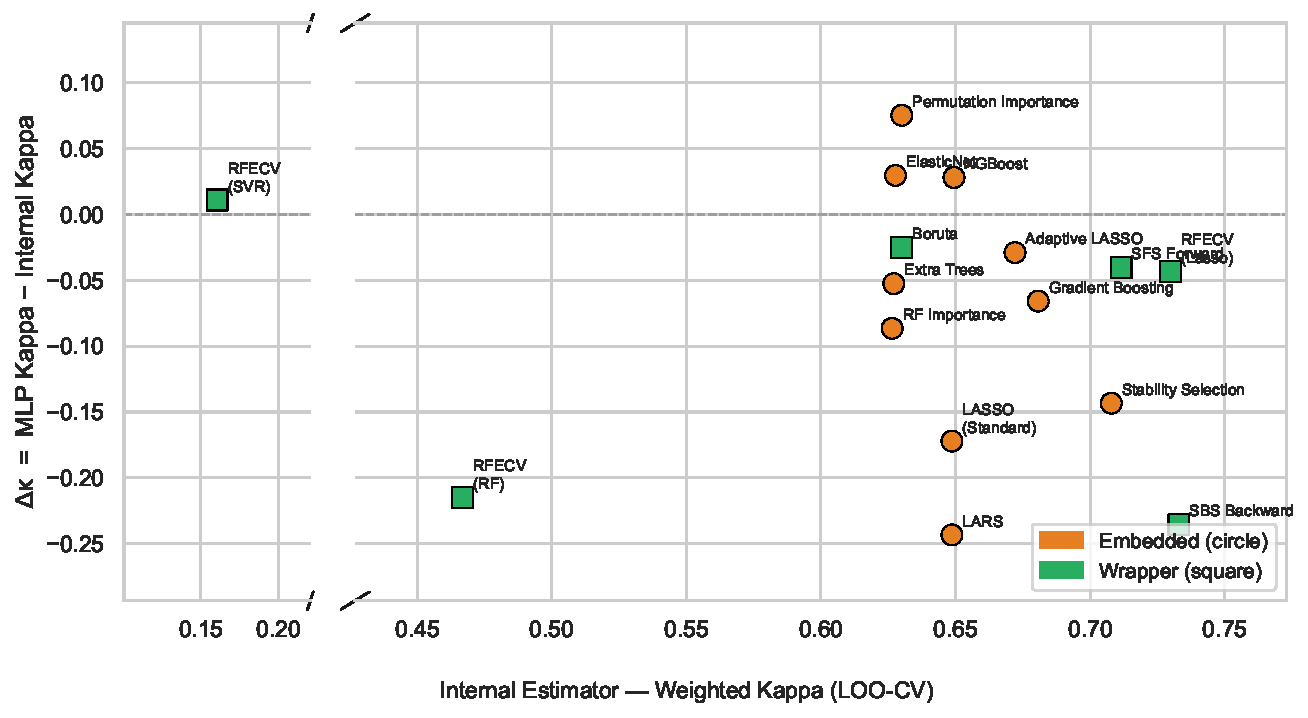
\includegraphics[width=\columnwidth]{figW4_kappa_delta}
    \caption{所有 16 種嵌入法（圓圈）與包裝法（方塊）在各自選取特徵上以 LOOCV 評估的
             $\Delta\kappa = \kappa_{\mathrm{MLP}} - \kappa_{\mathrm{int}}$
             對內部估計器 $\kappa$ 散佈圖。
             無任何方法落於左上象限（內部 $\kappa$ 低、$\Delta\kappa$ 高），
             確認 MLP 排名不受雜訊驅動選取的影響而膨脹。}
    \label{fig:wrap_vs_mlp}
\end{figure}

\subsection{LLM 評分效能}

表~\ref{tab:results} 呈現所有模型 $\times$ 設定組合的保留測試集效能。

\begin{table}[htbp]
    \centering
    \caption{模型效能（保留測試集，$n{=}53$，95\% 自助法信賴區間）}
    \label{tab:results}
    \renewcommand{\arraystretch}{1.2}
    \resizebox{\textwidth}{!}{%
    \begin{tabular}{llccc}
        \toprule
        \textbf{模型} & \textbf{設定} & \textbf{MAE}$\downarrow$ & \textbf{$\kappa$}$\uparrow$ & \textbf{AAcc}$\uparrow$ \\
        \midrule
        \multicolumn{5}{l}{\textit{原始軌跡方法（重現 Chen~\cite{chen2024chatgpt} 方法）}} \\
        Gemini-Flash & 零樣本，原始軌跡  & 0.66 {[0.47, 0.87]} & 0.37 {[0.18, 0.56]}       & 0.87 {[0.77, 0.94]} \\
        Gemini-Flash & 少樣本，原始軌跡  & 0.77 {[0.57, 0.98]} & 0.39 {[0.10, 0.61]}       & 0.87 {[0.77, 0.94]} \\
        \midrule
        \multicolumn{5}{l}{\textit{共識特徵選取方法（本研究）}} \\
        Qw-2.5-72B  & 零樣本，共識特徵  & 0.75 {[0.58, 0.91]} & $-$0.03 {[$-$0.11, 0.00]} & 0.94 {[0.87, 1.00]} \\
        DS-R1-70B   & 零樣本，共識特徵  & 0.79 {[0.64, 0.94]} & 0.03 {[0.00, 0.08]}       & 0.96 {[0.91, 1.00]} \\
        DS-R1-32B   & 零樣本，共識特徵 v2& 0.62 {[0.47, 0.77]} & 0.35 {[0.13, 0.52]}      & 0.96 {[0.91, 1.00]} \\
        Qw-2.5-32B  & 少樣本，共識特徵  & 0.79 {[0.60, 0.98]} & 0.45 {[0.28, 0.60]}       & 0.87 {[0.77, 0.94]} \\
        DS-R1-70B   & 少樣本，標準 LASSO& 0.57 {[0.42, 0.72]} & 0.51 {[0.21, 0.69]}       & 0.98 {[0.94, 1.00]} \\
        Qw-2.5-72B  & 少樣本，共識特徵  & 0.53 {[0.36, 0.70]} & 0.54 {[0.29, 0.72]}       & 0.91 {[0.83, 0.96]} \\
        DS-R1-70B   & 少樣本，共識特徵  & 0.62 {[0.47, 0.77]} & 0.57 {[0.37, 0.70]}       & 0.96 {[0.91, 1.00]} \\
        \textbf{DS-R1-32B} & \textbf{少樣本，共識特徵 v2} & \textbf{0.36 {[0.23, 0.49]}} & \textbf{0.68 {[0.53, 0.81]}} & \textbf{0.98 {[0.94, 1.00]}} \\
        \midrule
        \rowcolor{gray!15} 神經科醫師 X & 人類 & 0.40 {[0.26, 0.53]} & 0.69 {[0.50, 0.80]} & 1.00 {[1.00, 1.00]} \\
        \rowcolor{gray!15} 神經科醫師 Y & 人類 & 0.36 {[0.23, 0.49]} & 0.83 {[0.73, 0.89]} & 1.00 {[1.00, 1.00]} \\
        \rowcolor{gray!15} 均勻隨機     & 基線 & 1.46 {[1.19, 1.75]} & $-$0.00 {[$-$0.21, 0.21]} & 0.55 {[0.42, 0.68]} \\
        \rowcolor{gray!15} 比例隨機     & 基線 & 0.96 {[0.75, 1.17]} & $-$0.00 {[$-$0.26, 0.26]} & 0.75 {[0.64, 0.85]} \\
        \bottomrule
    \end{tabular}}
    \\[0.3em]
    {\small 少樣本\,=\,few-shot，零樣本\,=\,zero-shot；\colorbox{gray!15}{\phantom{x}} 為基線}
\end{table}

\begin{figure}[htbp]
    \centering
    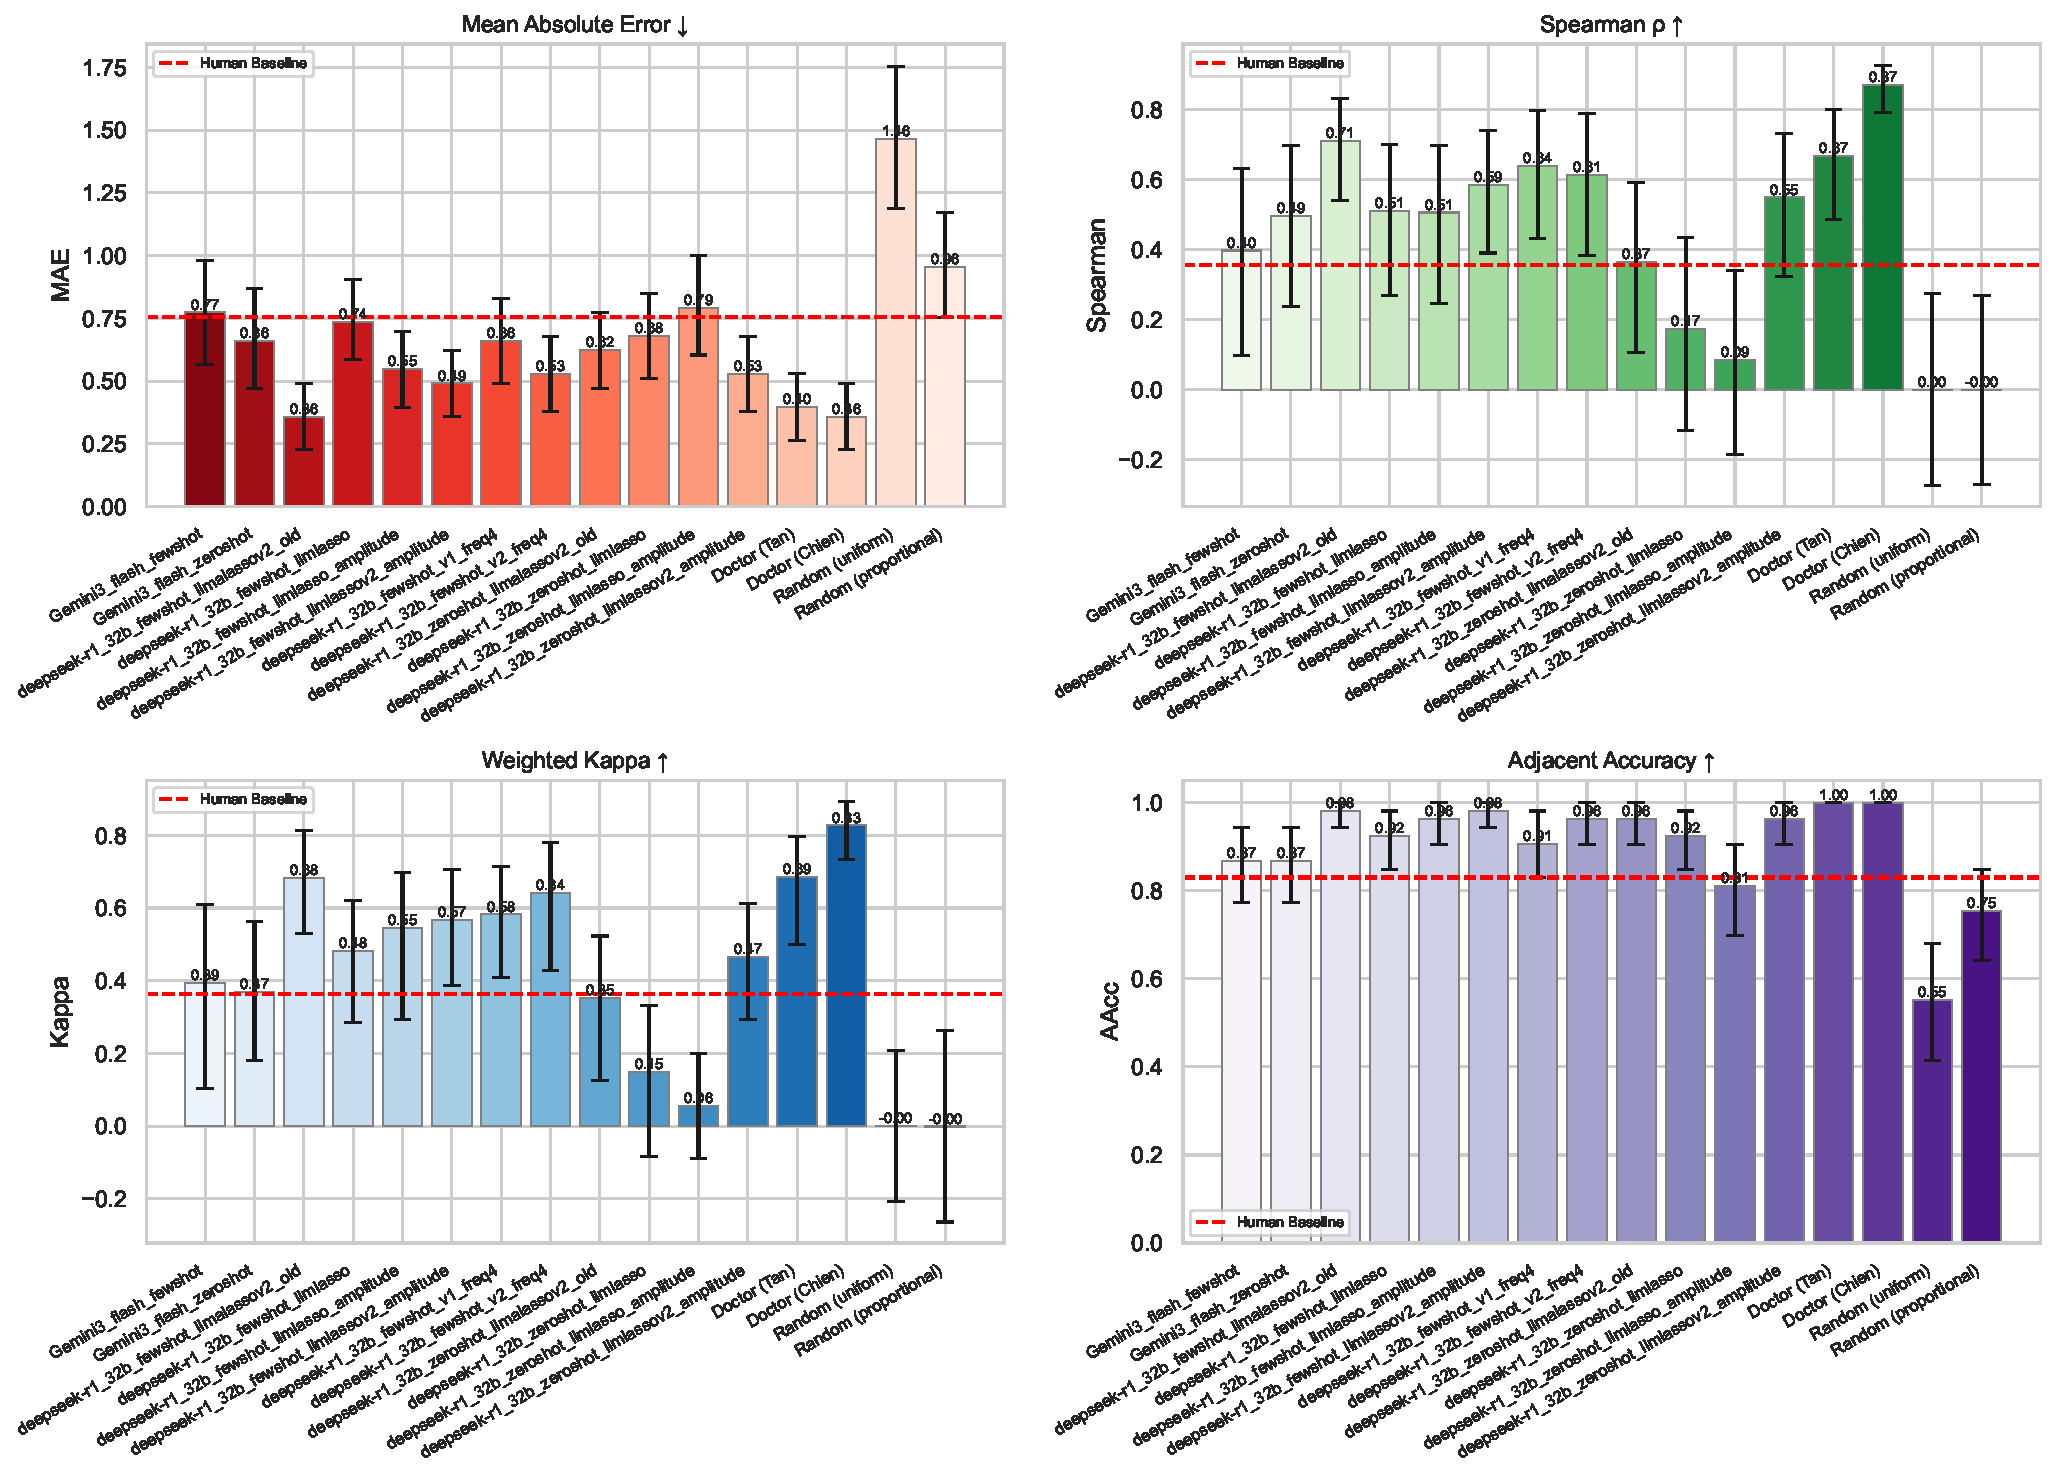
\includegraphics[width=\textwidth]{grouped_barplot}
    \caption{各模型在 MAE、加權 $\kappa$ 與相鄰準確率上的比較。灰色條代表人類專家基線。}
    \label{fig:barplot}
\end{figure}

主要觀察結果：
\begin{enumerate}
    \item \textbf{共識特徵選取 vs.\ 原始軌跡（受控比較）}：Gemini Flash 採用 Chen 的原始軌跡方法（少樣本）達到 $\kappa$\,=\,0.39、MAE\,=\,0.77。本研究共識特徵方法搭配 DS-R1-32B 達到 $\kappa$\,=\,0.68、MAE\,=\,0.36——$\kappa$ 提升 0.29、MAE 降低 52\%，顯示效能差距源自精簡且具臨床意義的特徵輸入，而非單純的模型選擇。
    \item \textbf{DS-R1-32B 少樣本達到人類專家水準}：MAE\,=\,0.36 與神經科醫師 Y（0.36）相當，$\kappa$\,=\,0.68 接近神經科醫師 X（0.69），為所有配置中最佳的 AI 結果。
    \item \textbf{共識特徵 v2 在參數更少的情況下優於 v1}：DS-R1-32B 少樣本-共識 v2（$\kappa$\,=\,0.68，32B）超越 DS-R1-70B 少樣本-共識（$\kappa$\,=\,0.57，70B），確認更強的特徵先驗可降低所需的模型容量。
    \item \textbf{零樣本評分持續失敗}：DS-R1-70B 零樣本（$\kappa$\,=\,0.03）與 Qw-2.5-72B 零樣本（$\kappa$\,=\,$-$0.03）均顯示，少樣本範例是可靠序數評分的硬性需求。
\end{enumerate}

\subsection{二元分類：正常 vs.\ 異常}

臨床上，區分未受影響受試者（評分\,=\,0）與任何異常手指敲擊（評分\,$\geq$\,1）是首要篩選決策。我們將預測重新歸為二元問題，並在表~\ref{tab:binary} 中回報準確率、召回率、精準率與 F1。

\begin{table}[htbp]
    \centering
    \caption{二元分類：正常（0）vs.\ 異常（$\geq$1）}
    \label{tab:binary}
    \renewcommand{\arraystretch}{1.2}
    \begin{tabular}{llcccc}
        \toprule
        \textbf{類型} & \textbf{模型} & \textbf{準確率} & \textbf{召回率} & \textbf{精準率} & \textbf{F1} \\
        \midrule
        \rowcolor{gray!15} ML & 隨機森林 & 79.2\% & 89.2\% & 82.5\% & 85.7\% \\
        \rowcolor{gray!15} ML & XGBoost  & 73.6\% & 89.2\% & 76.7\% & 82.5\% \\
        \midrule
        Chen~\cite{chen2024chatgpt} & Gemini3 Flash 零樣本 & 75.5\% & 73.2\% & 93.8\% & 82.2\% \\
        \midrule
        LLM & DS-R1-32B 少樣本 & \textbf{86.8\%} & \textbf{100.0\%} & \textbf{85.4\%} & \textbf{92.1\%} \\
        LLM & DS-R1-32B 零樣本 & 77.4\% & \textbf{100.0\%} & 77.4\% & 87.2\% \\
        LLM & DS-R1-70B 少樣本 & 83.0\% & 92.7\% & 86.4\% & 89.4\% \\
        LLM & DS-R1-70B 零樣本 & 81.1\% & \textbf{100.0\%} & 80.4\% & 89.1\% \\
        \bottomrule
    \end{tabular}
    \\[0.3em]
    {\small ML 基線以留一法交叉驗證評估。}
\end{table}

DS-R1-32B 少樣本達到最佳平衡：86.8\% 準確率與 100\% 召回率，即無任何異常 session 被漏判——對篩選工具而言是臨床上最重要的特性。所有 DeepSeek-R1 配置在每個指標上均超越 ML 基線及原始軌跡重現結果，且 32B 開源模型在使用約少 7 倍輸入 token 的情況下，F1 比 Chen 方法提升 $+$9.9 個百分點。

\subsection{Token 效率分析}

表~\ref{tab:tokens} 彙整各特徵配置的每 session 資料 token 成本。

\begin{table}[htbp]
    \centering
    \caption{提示詞 Token 消耗比較}
    \label{tab:tokens}
    \renewcommand{\arraystretch}{1.2}
    \begin{tabular}{lcc}
        \toprule
        \textbf{配置} & \textbf{Session 資料 Token（估計）} & \textbf{相對成本} \\
        \midrule
        Chen~\cite{chen2024chatgpt}（原始 CSV，四樣本少樣本）& $\sim$75\,800 & 75\,800\% \\
        Chen~\cite{chen2024chatgpt}（原始 CSV，零樣本）       & $\sim$15\,000 & 15\,000\% \\
        完整特徵集（95 個特徵）                               & $\sim$1\,900  &  1\,900\% \\
        標準 LASSO（11 個特徵）                               & $\sim$220     &    220\% \\
        \textbf{共識選取（6 個特徵，本研究）}                 & $\mathbf{\sim}$\textbf{100} & \textbf{100\%} \\
        \bottomrule
    \end{tabular}
\end{table}

相對於 Chen~\cite{chen2024chatgpt} 的原始軌跡方法（零樣本約 15\,000、少樣本約 75\,800 個 session token），預先萃取特徵使 session 資料 token 降低 \textbf{97\%} 至約 50--100 個。即便與傳入所有 95 個預萃取特徵相比（約 1\,900 個 token），共識選取仍可進一步降低 \textbf{95\%}。以規模化場景計算（每月 10\,000 次評估），此大幅降低可按比例削減推論成本——同時在原始軌跡基線上\emph{提升}預測品質（$\kappa$\,=\,0.68 vs.\ ICC\,=\,0.45）。

\subsection{消融實驗：特徵選取的作用}

將 MAE 對不同輸入特徵數作圖，在 6 個特徵處出現明顯的「手肘」彎折。超過 6 個特徵後，CV-MAE 單調遞增，確認額外特徵帶入的是雜訊而非有用訊號。

% -------------------------------------------------------
\section{討論}

\subsection{特徵預萃取為何能改善 LLM 推理}
原始軌跡方法~\cite{chen2024chatgpt} 要求 LLM 同時解析時間序列資料、執行情境內特徵萃取，並將結果對應至臨床評量準則——即便是 GPT-4 也因此受限（ICC\,=\,0.45）。本研究的方法解耦這些步驟：特徵萃取離線完成，選取透過 28 種方法的統計共識處理，LLM 只接收 7 個最具臨床相關性的特徵——直接對應 MDS-UPDRS 項目 3.4 的評估準則（幅度、速度、節律、停頓）。這種預先篩選解釋了為何 32B 開源模型搭配本方法的輸入能夠超越同一資料上的 GPT-4：呈現給模型的任務本身就更為簡單。

\subsection{少樣本是必要條件，而非選項}
零樣本結果（$\kappa \approx 0.03$ 至 $-0.03$）顯示，缺乏具體參考範例時，LLM 無法可靠地將運動學特徵值對應至 MDS-UPDRS 序數量表。少樣本範例錨定了評分尺度：向模型展示「\texttt{finger\_mvmnt\_x\_mean} = 0.12\,cm 且週期熵高 = 評分 2」的對應關係。這與臨床自然語言處理研究的發現一致：參考範圍範例對醫療情境中的數值推理至關重要~\cite{cite_clinicalnlp}。

\subsection{較小模型，更優效能}
最強的單一模型結果來自 Deepseek-R1-32B（32B 參數）少樣本配置（$\kappa$\,=\,0.68，MAE\,=\,0.36），優於所有 70B 變體與 Qwen 2.5-72B。這是一個引人注目的發現：在搭配更強特徵先驗的情況下，參數更少的模型超越了規模更大的對手。實際意涵相當重要：32B 參數的模型可部署於消費級 GPU 或院內伺服器，無需外部 API 存取，從而解決病患資料的隱私疑慮。

\subsection{研究限制}
\begin{itemize}
    \item 最佳 AI 模型（DS-R1-32B 少樣本，$\kappa$\,=\,0.68）接近但尚未達到較強人類專家的水準（神經科醫師 Y，$\kappa$\,=\,0.83），特別是在嚴重病例（評分 3--4）方面，模型傾向系統性低估。
    \item 少樣本方法需要人工整理參考範例；針對新任務建立這些範例需要臨床人員介入。
    \item 共識門檻（$\kappa \geq 0.5$、$|\mathcal{S}| < 15$）為啟發式設定；不同門檻可能改變合格方法集與最終共識特徵。
    \item 資料集規模（$n = 53$，來自 16 位患者）較小；需要更大規模研究以驗證普適性。
\end{itemize}

% -------------------------------------------------------
\section{結論}

本文提出一種節省 token 的 LLM 流程，用於 MDS-UPDRS 手指敲擊評估的自動化。透過以 CoTracker 萃取軌跡、建立 149 個運動學特徵池（七組 A--G），並以 28 種特徵選取方法的交叉共識壓縮至 7 個特徵，相較原始 CSV 提示達到 97\% 的 session 資料 token 減少。以共識特徵進行少樣本提示，使 Deepseek-R1-32B（32B 參數）達到 MAE\,=\,0.36、加權 $\kappa$\,=\,0.68——與人類專家 MAE 相當並接近評分者間 $\kappa$（0.69--0.83），同時可部署於單一消費級 GPU 且無需外部 API。在二元篩選任務上，DS-R1-32B 少樣本達到 100\% 召回率，零漏判。值得注意的是，此 32B 模型優於 70B 對手，顯示精簡且具臨床意義的特徵輸入可取代原始模型容量。本框架具任務通用性，適用於任何使用 LLM 對表格運動學輸入進行評分的臨床評估。未來研究將探討更大的患者群體、少樣本範例的領域適應，以及延伸至其他 MDS-UPDRS 動作子測驗。

% -------------------------------------------------------
\section*{致謝}
\textit{（待填入）}

% -------------------------------------------------------
\begin{thebibliography}{99}

\bibitem{Peng2005}
H.~Peng, F.~Long, and C.~Ding,
``Feature selection based on mutual information: criteria of max-dependency,
max-relevance, and min-redundancy,''
\textit{IEEE Trans.\ Pattern Anal.\ Mach.\ Intell.}, vol.~27, no.~8,
pp.~1226--1238, 2005.

\bibitem{Meinshausen2009}
N.~Meinshausen and P.~B\"{u}hlmann,
``Stability selection,''
\textit{Journal of the Royal Statistical Society: Series B}, vol.~72, no.~4,
pp.~417--473, 2010.

\bibitem{steinmetz2024global}
G.~A. Steinmetz et al.,
``Global, regional, and national burden of disorders affecting the nervous
system, 1990--2021: a systematic analysis for the Global Burden of Disease
Study 2021,''
\textit{The Lancet Neurology}, vol.~23, no.~4, pp.~344--381, 2024.

\bibitem{sarker2022ai}
I.~H. Sarker,
``AI-Based Modeling: Techniques, Applications and Research Issues
Towards Automation, Intelligent and Smart Systems,''
\textit{SN Computer Science}, vol.~3, p.~158, 2022.

\bibitem{minaee2024large}
S.~Minaee et al.,
``Large Language Models: A Survey,''
arXiv:2402.06196, 2024.

\bibitem{tibshirani1996}
R. Tibshirani,
``Regression shrinkage and selection via the lasso,''
\textit{Journal of the Royal Statistical Society: Series B}, vol.~58, no.~1,
pp.~267--288, 1996.

\bibitem{cite_updrs}
C.~G. Goetz et al.,
``Movement Disorder Society-sponsored revision of the Unified Parkinson's Disease
Rating Scale (MDS-UPDRS): scale presentation and clinimetric testing results,''
\textit{Movement Disorders}, vol.~23, no.~15, pp.~2129--2170, 2008.

\bibitem{cite_fewshot}
T.~Brown et al.,
``Language models are few-shot learners,''
in \textit{Proc.\ NeurIPS}, 2020.

\bibitem{cite_ml_motor}
N.~Yang et al.,
``Automatic Detection Pipeline for Accessing the Motor Severity of
Parkinson's Disease in Finger Tapping and Postural Stability,''
\textit{IEEE Access}, vol.~10, pp.~66961--66971, 2022.

\bibitem{cite_ml_motor2}
T.~Yu, K.~W. Park, M.~J. McKeown, and Z.~J. Wang,
``Clinically Informed Automated Assessment of Finger Tapping Videos
in Parkinson's Disease,''
\textit{Sensors}, vol.~23, no.~22, p.~9149, 2023.

\bibitem{cite_gpt4clinical}
Z.~Gu, W.~Jia, M.~Piccardi, and P.~Yu,
``Empowering Large Language Models for Automated Clinical Assessment
with Generation-Augmented Retrieval and Hierarchical Chain-of-Thought,''
\textit{Artificial Intelligence in Medicine}, vol.~162, p.~103078, 2025.

\bibitem{cite_weighted_lasso}
H.~Zou,
``The Adaptive Lasso and Its Oracle Properties,''
\textit{Journal of the American Statistical Association},
vol.~101, no.~476, pp.~1418--1429, 2006.

\bibitem{cite_clinicalnlp}
Z.~Gu, W.~Jia, M.~Piccardi, and P.~Yu,
``Empowering Large Language Models for Automated Clinical Assessment
with Generation-Augmented Retrieval and Hierarchical Chain-of-Thought,''
\textit{Artificial Intelligence in Medicine}, vol.~162, p.~103078, 2025.

\bibitem{vanbelle2016}
S.~Vanbelle,
``A New Interpretation of the Weighted Kappa Coefficients,''
\textit{Psychometrika}, vol.~81, no.~2, pp.~399--410, 2016.

\bibitem{yang2024deep}
J.~Yang, S.~Williams, D.~C. Hogg, J.~E. Alty, and S.~D. Relton,
``Deep Learning of Parkinson's Movement from Video, Without
Human-Defined Measures,''
\textit{Journal of the Neurological Sciences}, vol.~463, p.~123089, 2024.

\bibitem{li2021automated}
Z.~Li et al.,
``Automated Assessment of Finger-Tapping with Smartphone Videos,''
\textit{IEEE Access}, vol.~9, pp.~165914--165929, 2021.

\bibitem{chen2024chatgpt}
D. Chen,
``Evaluating ChatGPT-4 for MDS-UPDRS Finger Tapping Severity Assessment,''
M.Sc.\ Thesis, Dept.\ of Mechanical Engineering,
National Cheng Kung University, Tainan, Taiwan, 2024.

\bibitem{ashyani2022digitization}
M. Ashyani et al.,
``Digitization of Parkinson's Disease Assessment: A Multi-test Smartphone
Protocol for Motor Evaluation,''
\textit{Sensors}, vol.~22, no.~11, p.~4160, 2022.

\bibitem{karaev2023cotracker}
N. Karaev, G. Rocco, B. Graham, N. Neverova, A. Vedaldi, and C. Rupprecht,
``CoTracker: It Is Better to Track Together,''
in \textit{Proc.\ ECCV}, 2024.

\bibitem{goetz2004movement}
C.~G. Goetz et al.,
``Movement Disorder Society Task Force Report on the Hoehn and Yahr Staging
Scale: Status and Recommendations,''
\textit{Movement Disorders}, vol.~19, no.~9, pp.~1020--1028, 2004.

\bibitem{DeepSeek2025R1}
DeepSeek-AI,
``DeepSeek-R1: Incentivizing Reasoning Capability in LLMs via Reinforcement
Learning,''
arXiv:2501.12948, Jan.\ 2025.

\end{thebibliography}

\end{document}
